\chapter{Conception générale}

\section{Répartition en paquetage}

Dans notre projet, nous avons un paquetage par défaut \textit{stockgestion}. Dans ce paquetage, nous retrouvons 5 sous-paquetages \textit{Entite}, \textit{Manager}, \textit{Controlleur}, \textit{Outil} et \textit{UI}.\\

Voici notre diagramme de classe dans sa version finale, avec les relations entre les paquetages.

\begin{center}
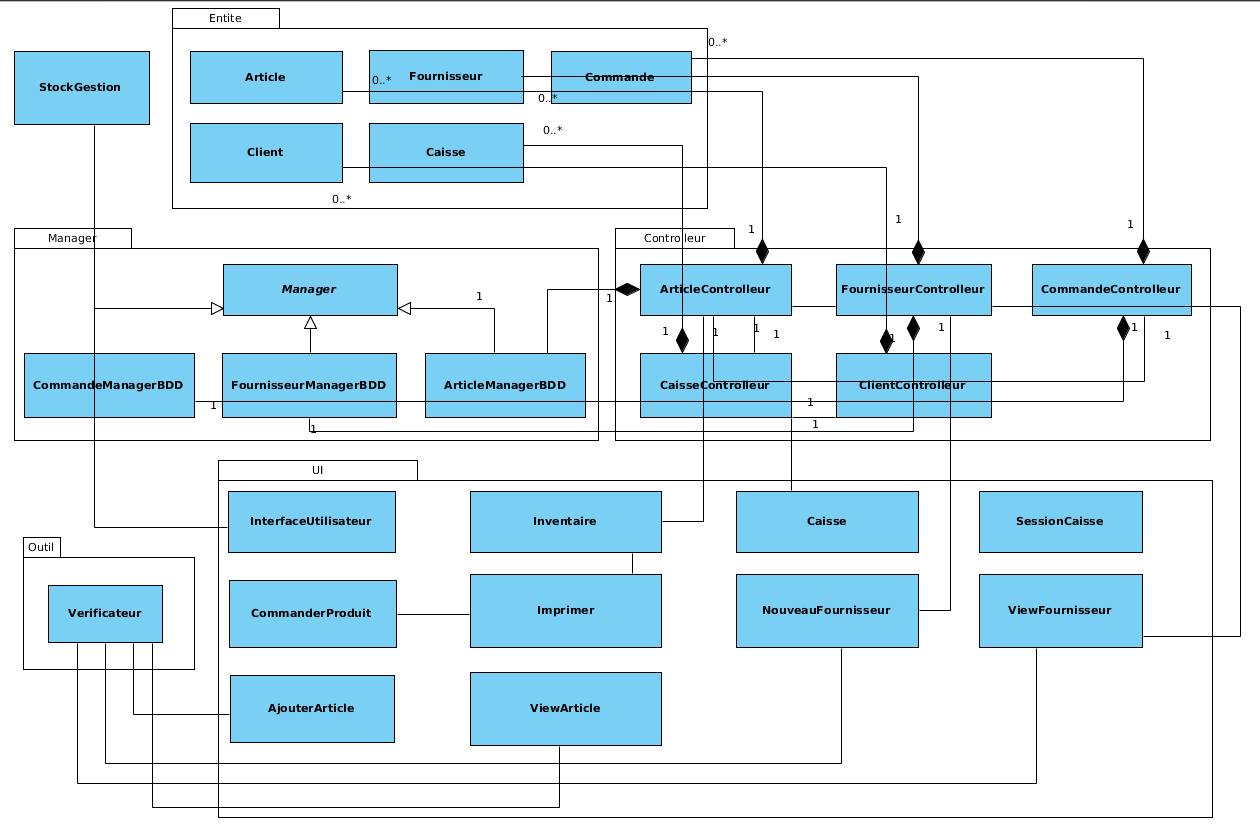
\includegraphics[width=14cm]{./Conception/DiagrammeDeClassePackage}
\end{center}


\section{Les choix technologiques}

\section{Diagramme de composant du logiciel}

\section{Diagramme de déploiement}



\chapter{Conception détaillée}

\section{Diagrammes de classes techniques des paquetages}

A la racine de notre projet, nous retrouvons le paquetage \textbf{stockgestion} créé par défaut. Ce paquetage ne contient qu'une seule classe \textbf{StockGestion} qui a le rôle d'initialiser et de rafraîchir toutes les interfaces d'utilisateur lors des changements dans les données.

\begin{center}
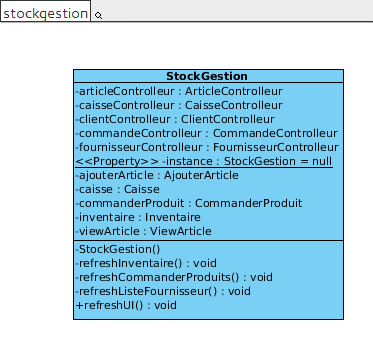
\includegraphics[width=14cm]{./Conception/stockgestion}
\end{center}

Dans le paquetage \textbf{stockgestion}, nous retrouvons 5 sous-paquetages, chacun contient des classes qui jouent un certain rôle précis dans l'application.\\

Premièrement, nous avons le paquetage \textbf{Entite}. Dans ce paquetage, chaque classe représente une entité utilisé dans l'application: un article, un fournisseur, une commande, un client ou encore une caisse.

\begin{center}
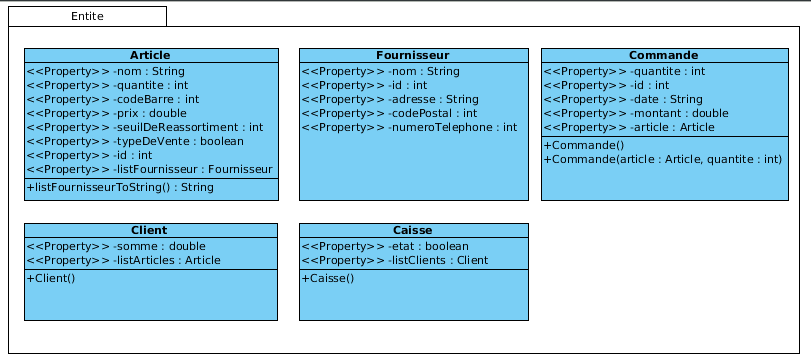
\includegraphics[width=14cm]{./Conception/entite}
\end{center}

Ensuite, nous avons le paquetage \textbf{Manager}. Chaque classe dans ce paquetage s'occupe de la connexions avec la base de données ainsi que de toutes les opérations liées à cette base.\\
Nous retrouvons ici la classe mère \textbf{Manager} qui contient la méthode de connexion à Derby. Nous avons 3 classes filles, chacune s'occupe des opération des articles, des commandes et des fournisseurs respectivement.

\begin{center}
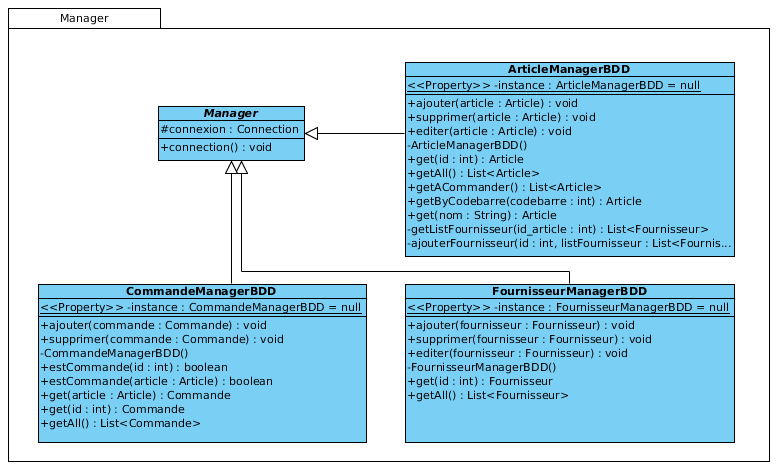
\includegraphics[width=14cm]{./Conception/manager}
\end{center}

Nous avons le paquetage \textbf{Controleur} qui contient des classes de contrôleurs. Ces classes réalisent les opérations sur les entités en appelant les méthodes des managers.

\begin{center}
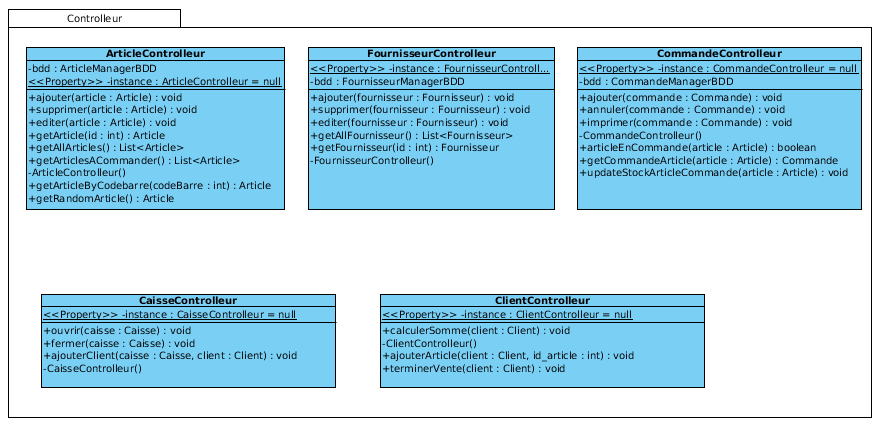
\includegraphics[width=14cm]{./Conception/controlleur}
\end{center}

Pour les besoins très spécifiques de notre application, nous avons créé le paquetage \textbf{Outil}. Dedans on trouve la classe \textbf{Verificateur} qui s'occupe de toutes les vérifications des entrées utilisateurs de notre application, ainsi permet d'éviter des erreurs avec la base de données (un numéro mal écrit, un texte avec des caractères spéciaux...).

\begin{center}
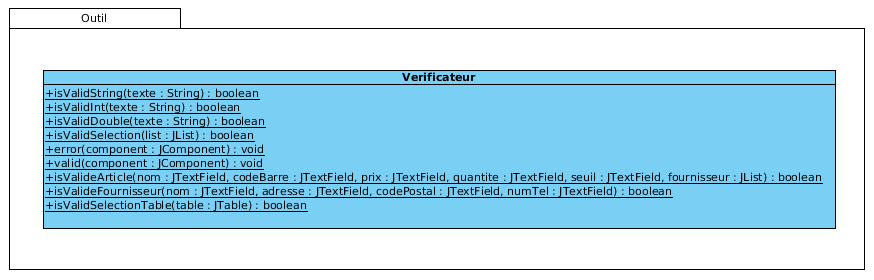
\includegraphics[width=14cm]{./Conception/outil}
\end{center}

Enfin, nous avons le paquetage \textbf{UI} qui contient toutes les classes de notre interface utilisateur. Chaque classe représente une fenêtre différente, chaque fenêtre correspond à une fonctionnalité de notre application.

\begin{center}
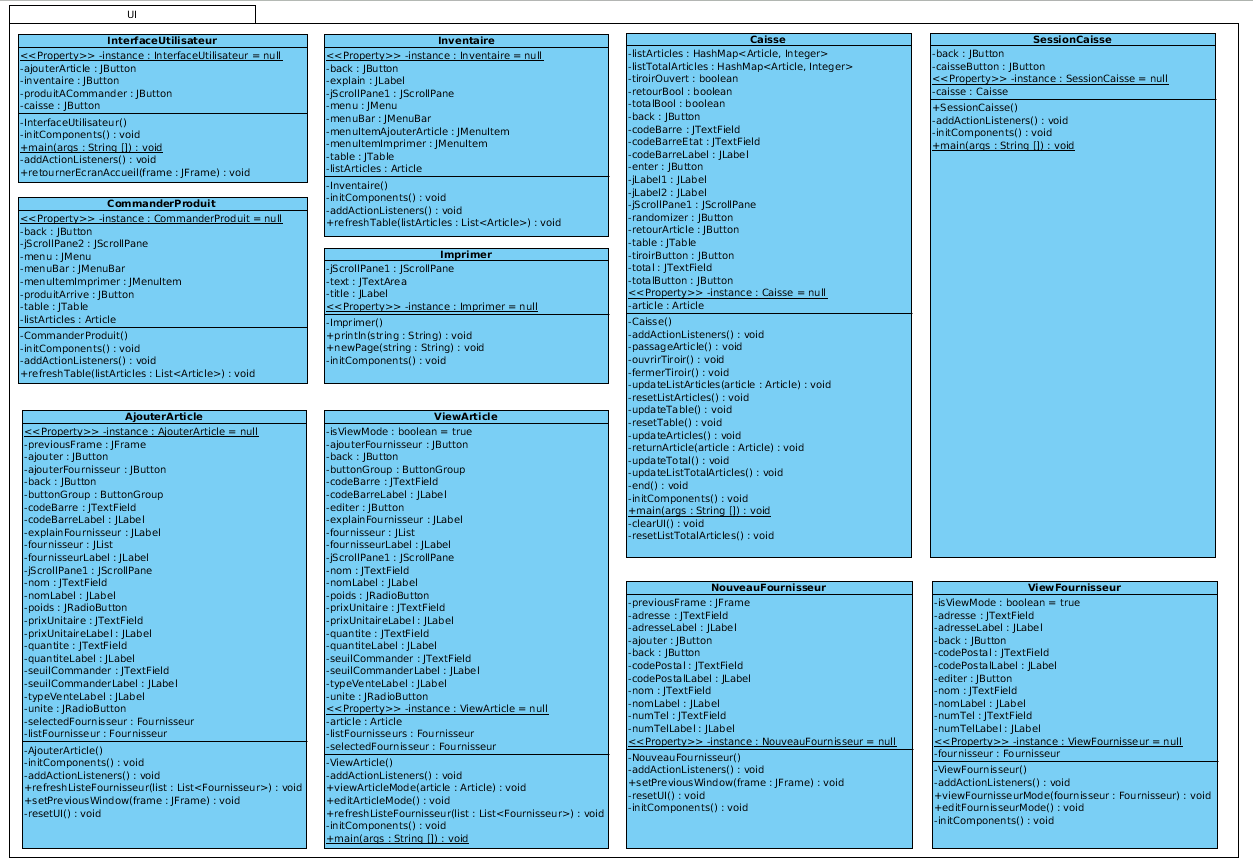
\includegraphics[width=14cm]{./Conception/ui}
\end{center}


\section{Diagrammes de séquences techniques}

\section{Architecture du projet: approche MVC}


\chapter{Phase d'implémentation}